\chapter{Introducción}
\label{cap:introduccion}
\setcounter{page}{1}

El avance tecnológico constante ha transformado nuestra forma de percibir el mundo. Tecnologías como la robótica han dado lugar a dispositivos capaces de realizar tareas que antes parecían imposibles. Hace medio siglo, la idea de un aparato que pudiera barrer de manera eficiente o de un vehículo que se condujera solo era pura fantasía. Hoy, los vehículos inteligentes han pasado de ser un concepto de ciencia ficción a convertirse en una realidad que está revolucionando el transporte y remodelando nuestras ciudades.

La capacidad de los vehículos autónomos para desenvolverse de manera segura en entornos complejos, no solo reducen los errores humanos, sino que también abren nuevas oportunidades en ámbitos esenciales. Desde mejorar la seguridad vial y promover la eficiencia energética hasta fomentar la inclusión social, convirtiéndose en pilares fundamentales para el desarrollo de ciudades más sostenibles. Aunque todavía queda un largo camino por recorrer, estos avances permiten vislumbrar un futuro donde el tráfico sea más fluido, los recursos urbanos estén mejor aprovechados y las personas con movilidad reducida o dificultades para conducir tengan un acceso más equitativo a los servicios de transporte.

En este \ac{TFG}, nos centraremos en los sistemas de conducción autónoma, explorando su aplicación en la movilidad inteligente dentro de entornos urbanos. Analizaremos cómo la \ac{IA} contribuye a este campo, tanto en el aspecto sensorial como en el de control. En el ámbito del control, nos enfocaremos en \ac{DRL}, evaluando diferentes algoritmos para determinar cuáles ofrecen los mejores resultados.

\section{Vehículos autónomos}
\label{sec:vehículos}

Un vehículo autónomo es aquel capaz de realizar todas las funciones de conducción entre un origen y un destino sin la intervención de un ser humano, más allá de indicar el punto de inicio y final del trayecto. En los niveles intermedios, donde aún se requiere la actuación de un conductor, la autonomía no es total.

En la actualidad, la industria automotriz ha desarrollado una amplia gama de \ac{ADAS}, cuyo objetivo principal es reducir el riesgo de accidentes. Estos sistemas utilizan una red de sensores para analizar el entorno de conducción, procesando la información mediante la electrónica del vehículo. Con esta información, el sistema toma decisiones predefinidas y puede intervenir en elementos como el acelerador, los frenos o la dirección. Entre sus funcionalidades más comunes hoy en día se incluyen aquellos que corrigen desvíos involuntarios del carril o alertan al conductor sobre peligros inminentes que requieren una respuesta inmediata. Aunque estos avances representan pasos intermedios hacia la conducción autónoma completa, los \ac{ADAS} continúan asistiendo al conductor en tareas específicas, aunque aún requieren su supervisión activa. No solo mejoran la seguridad en los vehículos actuales, sino que también establecen las bases para la implementación futura de sistemas totalmente autónomos.

La Sociedad de Ingenieros Automotrices (\ac{SAE}) ha establecido una clasificación estandarizada de los niveles de autonomía de los vehículos, que abarca desde la conducción completamente manual hasta la conducción completamente autónoma. Esta categorización divide los vehículos autónomos en seis niveles, según el grado de intervención que se requiere del conductor y la capacidad del sistema del vehículo para tomar control \cite{autobild-autonomous}.

\begin{figure} [ht]
  \begin{center}
    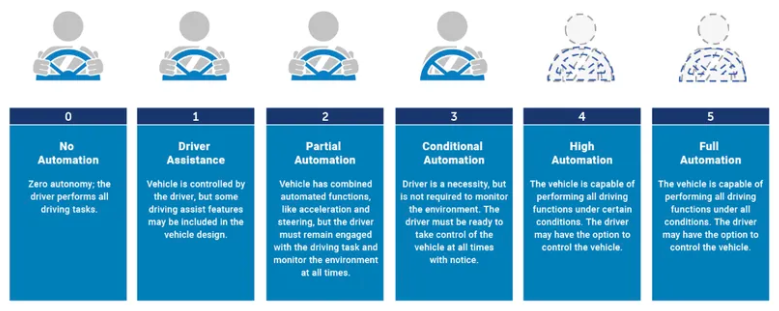
\includegraphics[width=12cm]{figs/introducción/niveles.png}
  \end{center}
  \caption{Niveles de autonomía explicados(\ac{SAE}).}
  \label{aut-levels}
  \end{figure}

\begin{itemize}
    \item \textit{Nivel 0:} Ninguna autonomía. El conductor es completamente responsable de todas las tareas de conducción.
    \item \textit{Nivel 1:} Asistencia al conductor. El vehículo puede realizar una función específica (como el control de crucero), pero siempre requiere la supervisión activa del conductor.
    \item \textit{Nivel 2:} Automatización parcial. El vehículo cuenta con sistemas que pueden replicar tareas del conductor, pero el conductor debe estar preparado para intervenir en cualquier momento.
    \item \textit{Nivel 3:} Automatización condicional. El vehículo puede tomar control completo en determinadas condiciones, pero el conductor debe estar disponible para retomar el control si el sistema lo solicita. Un ejemplo destacado de este nivel es el Autopilot de Tesla \footnote{\url{https://www.tesla.com/es_es/support/autopilot}}.
    \item \textit{Nivel 4:} Alta automatización. El vehículo puede operar de forma autónoma en condiciones específicas, sin necesidad de intervención humana, aunque pueden existir limitaciones geográficas o contextuales.
    \item \textit{Nivel 5:} Automatización total. El vehículo es completamente autónomo y no requiere intervención humana en ningún momento ni bajo ninguna circunstancia.
\end{itemize}

Hoy en día, no existen vehículos completamente autónomos disponibles comercialmente. Lo más cercano a la autonomía total que se puede encontrar en el mercado es el nivel 2+. Sin embargo, existen numerosos proyectos en desarrollo que están alcanzando el nivel 3, como es posible ver videos promocionales que muestran coches en movimiento sin intervención activa del conductor. No obstante, estas demostraciones se realizan en entornos extremadamente controlados y con condiciones específicas.

En algunos países, la legislación aún no permite el uso de vehículos autónomos de nivel 3 o superior. Por ejemplo, en España, la ley prohíbe que el conductor suelte el volante durante la conducción, lo que impide el uso de vehículos de nivel 3. En cambio, en California, es legal el uso de vehículos con conducción semi-autónoma, lo que permite al conductor levantar las manos del volante en ciertas circunstancias \cite{carwow-autonomous}.

\subsection{Evolución histórica de los vehículos autónomos}
\label{sec:historia}

La primera vez que se puso en práctica el concepto de vehículo autónomo fue en 1925 en Nueva York. El ingeniero Francis Houdina diseñó el primer coche sin conductor, controlado de forma remota por radiofrecuencia. Sin embargo, este vehículo requería un coche escolta desde el cual se dirigía.

En 1939, el diseñador industrial estadounidense Norman Bel Geddes revolucionó las ideas sobre transporte al presentar, en la Feria Futurama, un concepto visionario: vehículos eléctricos guiados de manera autónoma mediante radiocontrol en carreteras automáticas con circuitos eléctricos integrados en el pavimento. Aunque no se trataba del concepto moderna de coche autónomo, esta propuesta marcó un antes y un después, despertando el interés de numerosas empresas tecnológicas en el campo de la conducción autónoma.

\begin{figure} [ht]
  \begin{center}
    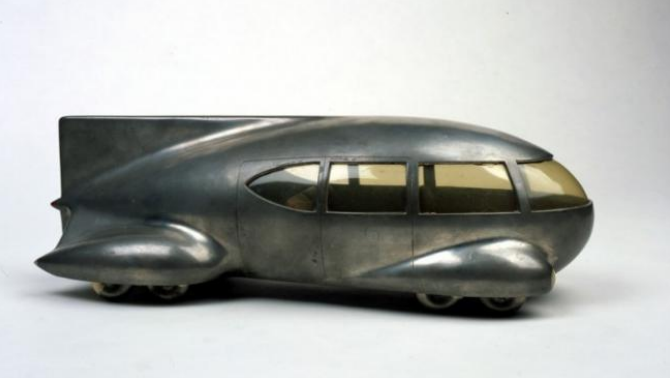
\includegraphics[width=12cm]{figs/introducción/coche_geddes.png}
  \end{center}
  \caption{Coche diseñado por Norman Bel Geddes en 1933.}
  \label{coche-geddes}
  \end{figure}

La mayoría de los avances significativos en este ámbito se deben a Ernst Dickmanns, un profesor alemán experto en \ac{IA}. Dickmanns lideró la creación del primer coche autónomo moderno, combinado la visión sacádica (un movimiento
rápido del ojo, cabeza u otras partes del cuerpo de animales o dispositivos) con cálculos probabilísticos y computación paralela. En 1987, diseñó una furgoneta \textit{Mercedes-Benz} equipada con esta tecnología, logrando conducirla exitosamente por una autopista a velocidades de hasta 100 km/h en condiciones de tráfico controladas. En 1994, lo superó con el modelo  \textit{Mercedes 500 SEL}, conocido como \textit{VaMP}, que recorrió más de 1.000 kilómetros en la carretera de circunvalación de París. Este vehículo alcanzó velocidades de hasta 130 km/h y era capaz de realizar maniobras complejas, como adelantamientos.

\begin{figure}[ht]
  \begin{center}
    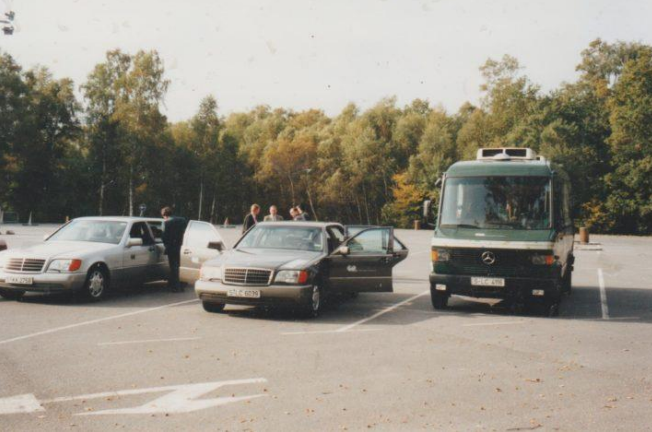
\includegraphics[width=9cm]{figs/introducción/paris_1994.png}
  \end{center}
  \caption{Demostración en vico del funcionamiento de \textit{VaMP} en París.}
  \label{coche-geddes}
\end{figure}

La Comisión Europea, consciente del potencial de los coches autónomos, destinó 800 millones de euros al proyecto  \textit{EUREKA Prometheus}, una iniciativa que marcó un hito en el desarrollo de esta tecnología. Este programa facilitó la creación de numerosos prototipos que sentaron las bases de los vehículos autónomos modernos  \cite{history-vehicles}. Actualmente, este campo es liderado por empresas pioneras como  \textit{Waymo},  \textit{Tesla},  \textit{Cruise} y  \textit{NVIDIA } \cite{ai-self-driving-cars}.

\subsection{Desafíos actuales en la implementación de vehículos autónomos}
\label{sec:desafíos}

Los vehículos autónomos enfrentan numerosos desafíos que deben ser superados para lograr su implementación generalizada. Estos desafíos se dividen principalmente en aspectos técnicos y no técnicos, cada uno con sus propias complejidades que requieren soluciones específicas.

En el ámbito técnico, uno de los mayores retos radica en la detección y análisis de datos. Los vehículos autónomos necesitan identificar obstáculos de manera inequívoca, incluso a altas velocidades y largas distancias. Esto exige un software avanzado capaz de procesar grandes volúmenes de datos en tiempo real con un alto grado de precisión, un área que aún enfrenta importantes limitaciones. Además, garantizar un sistema seguro y fiable implica desarrollar tecnología tolerante a fallos y capaz de operar de manera eficiente en entornos no controlados. En el mundo real, los vehículos autónomos deben enfrentarse a miles de situaciones impredecibles durante la conducción, y los sistemas actuales todavía están lejos de resolver de manera eficiente todas estas incertidumbres.

Otro desafío técnico crucial es la seguridad cibernética. Los vehículos autónomos, especialmente aquellos basados en \ac{DL}, son vulnerables a ataques que podrían comprometer su funcionalidad o la seguridad de sus ocupantes. Por ello, es imprescindible implementar estrategias robustas de defensa para mitigar estos riesgos y generar confianza en la tecnología.
En el ámbito no técnico, las cuestiones legales y éticas presentan una barrera importante. Existe una preocupación creciente sobre la responsabilidad en caso de accidentes, ya que no está claro si la culpa recaería en el fabricante, el desarrollador del software o el propietario del vehículo. También es esencial salvaguardar la privacidad de los datos de los pasajeros, ya que los sistemas autónomos recopilan y procesan grandes cantidades de información personal.

La aceptación por parte de los consumidores y las regulaciones gubernamentales son factores determinantes en el desarrollo de vehículos autónomos. En la actualidad, las políticas y normativas suelen avanzar a un ritmo más lento que el desarrollo tecnológico, lo que complica las pruebas y la implementación a gran escala.

La superación de estos obstáculos requerirá soluciones innovadoras que satisfagan las necesidades de los consumidores, la industria y los gobiernos. La colaboración interdisciplinaria será clave para abordar estos desafíos, sentando las bases de un futuro en el que los vehículos autónomos sean seguros, eficientes y ampliamente aceptados en la sociedad \cite{challenges-autonomous}.

\section{Impacto de la IA en el transporte autónomo}
\label{sec:ia-intro}
